% Template for Elsevier CRC journal article
% version 1.1-5p dated 18 January 2011
% SEM ACENTUACAO PROBLEMA UTF-8 : NAO ACEITA

% This file (c) 2010-2011 Elsevier Ltd.  Modifications may be freely made,
% provided the edited file is saved under a different name

% This file contains modifications for Procedia Computer Science
% but may easily be adapted to other journals

% Changes since version 1.0
% - elsarticle class option changed from 1p to 3p (to better reflect CRC layout)
% - this version uses option 5p for larger-format journals (text area 24.1 x 18.4 cm)

%-----------------------------------------------------------------------------------

%% This template uses the elsarticle.cls document class and the extension package ecrc.sty
%% For full documentation on usage of elsarticle.cls, consult the documentation "elsdoc.pdf"
%% Further resources available at http://www.elsevier.com/latex

%-----------------------------------------------------------------------------------

%%%%%%%%%%%%%%%%%%%%%%%%%%%%%%%%%%%%%%%%%%%%%%
%%%%%%%%%%%%%%%%%%%%%%%%%%%%%%%%%%%%%%%%%%%%%%
%%                                          %%
%% Important note on usage                  %%
%% -----------------------                  %%
%% This file must be compiled with PDFLaTeX %%
%% Using standard LaTeX will not work!      %%
%%                                          %%
%%%%%%%%%%%%%%%%%%%%%%%%%%%%%%%%%%%%%%%%%%%%%%
%%%%%%%%%%%%%%%%%%%%%%%%%%%%%%%%%%%%%%%%%%%%%%

%% The '5p' and 'times' class options of elsarticle are used for Elsevier CRC
\documentclass[5p,times]{elsarticle}

%% The `ecrc' package must be called to make the CRC functionality available
%% ecrc_RIAI es el paquete ecrc de Elsevier con modificaciones para la revista RIAI
\usepackage{ecrc_RIAI}

%% The ecrc package defines commands needed for running heads and logos.
%% For running heads, you can set the journal name, the volume, the starting page and the authors

%%%%%%%%%%%%%%%%%%%%%%%%%%%%%%%%% Aaadido por Secretaraa RIAI
%\usepackage[spanish]{babel}     % Idioma
%\addto{\captionsspanish}{\renewcommand{\abstractname}{Abstract}}
%\addto\captionsspanish{%
%\def\tablename{Tabla}%
%}
%\usepackage[latin1]{inputenc}   % Lengua latina
\usepackage{amsmath}            % Para las referencias a ecuaciones con \eqref
\usepackage{mathtools}
\newcommand{\defeq}{\vcentcolon=}
\newcommand{\eqdef}{=\vcentcolon}
\usepackage{epstopdf}           % Para poder insertar figuras .eps al compilar con PDFLATEX
\usepackage{flushend}           % Para igualar las columnas de la altima pagina
\usepackage{placeins}
%\usepackage{hyperref}           % Para hipervanculos dentro del PDF
%%%%%%%%%%%%%%%%%%%%%%%%%%%%%%%%%%%%%%%%%%%%%%%%%%%%%%%

%% set the volume if you know. Otherwise `00'
\volume{} 

%% set the starting page if not 1
\firstpage{1}

%% Give the name of the journal
\journalname{MA931 Individual Project}

%% Give the author list to appear in the running head
%% Example \runauth{C.V. Radhakrishnan et al.}
\runauth{Emma L Davis}

%% The choice of journal logo is determined by the \jid and \jnltitlelogo commands.
%% A user-supplied logo with the name <\jid>logo.pdf will be inserted if present.
%% e.g. if \jid{yspmi} the system will look for a file yspmilogo.pdf
%% Otherwise the content of \jnltitlelogo will be set between horizontal lines as a default logo

%% Give the abbreviation of the Journal. Contast the Publisher if in doubt what this is.
\jid{comp}

%% Give a short journal name for the dummy logo (if needed)
\jnltitlelogo{comp}

%% Hereafter the template follows `elsarticle'.
%% For more details see the existing template files elsarticle-template-harv.tex and elsarticle-template-num.tex.

%% Elsevier CRC generally uses a numbered reference style
%% For this, the conventions of elsarticle-template-num.tex should be followed (included below)
%% If using BibTeX, use the style file elsarticle-num.bst

%% End of ecrc-specific commands
%%%%%%%%%%%%%%%%%%%%%%%%%%%%%%%%%%%%%%%%%%%%%%%%%%%%%%%%%%%%%%%%%%%%%%%%%%

%% The amssymb package provides various useful mathematical symbols
\usepackage{amssymb}
%% The amsthm package provides extended theorem environments
%% \usepackage{amsthm}

%% The lineno packages adds line numbers. Start line numbering with
%% \begin{linenumbers}, end it with \end{linenumbers}. Or switch it on
%% for the whole article with \linenumbers after \end{frontmatter}.
%% \usepackage{lineno}

%% natbib.sty is loaded by default. However, natbib options can be
%% provided with \biboptions{...} command. Following options are
%% valid:

\biboptions{sort}

%\setcitestyle{number}

%%   round  -  round parentheses are used (default)
%%   square -  square brackets are used   [option]
%%   curly  -  curly braces are used      {option}
%%   angle  -  angle brackets are used    <option>
%%   semicolon  -  multiple citations separated by semi-colon
%%   colon  - same as semicolon, an earlier confusion
%%   comma  -  separated by comma
%%   numbers-  selects numerical citations
%%   super  -  numerical citations as superscripts
%%   sort   -  sorts multiple citations according to order in ref. list
%%   sort&compress   -  like sort, but also compresses numerical citations
%%   compress - compresses without sorting
%%
%% \biboptions{comma,round}

% \biboptions{}

% if you have landscape tables
\usepackage[figuresright]{rotating}

% put your own definitions here:
%   \newcommand{\cZ}{\cal{Z}}
%   \newtheorem{def}{Definition}[section]
%   ...

% add words to TeX's hyphenation exception list
%\hyphenation{author another created financial paper re-commend-ed Post-Script}

% para poder introducir varias figuras que ocupen el ancho de las dos columnas.
\usepackage{subfigure}

% declarations for front matter

\begin{document}
%\selectlanguage{english}

\begin{frontmatter}

%% Title, authors and addresses

%% use the tnoteref command within \title for footnotes;
%% use the tnotetext command for the associated footnote;

%% use the fnref command within \author or \address for footnotes;
%% use the fntext command for the associated footnote;

%% use the corref command within \author for corresponding author footnotes;
%% use the cortext command for the associated footnote;
%% use the ead command for the email address,
%% and the form \ead[url] for the home page:
%%
%% \title{Title\tnoteref{label1}}
%% \tnotetext[label1]{}
%% \author{Name\corref{cor1}\fnref{label2}}
%% \ead{email address}
%% \ead[url]{home page}
%% \fntext[label2]{}
%% \cortext[cor1]{}
%% \address{Address\fnref{label3}}
%% \fntext[label3]{}

%\dochead{Cabecera artaculo}
%% Use \dochead if there is an article header, e.g. \dochead{Short communication}

\title{Modelling the role of long lasting insecticide-treated bednets in the reduction of lymphatic filariasis prevalence in The Gambia}


%% use optional labels to link authors explicitly to addresses:
%% \author[label1,label2]{<author name>}
%% \address[label1]{<address>}
%% \address[label2]{<address>}

\author[First]{Emma L Davis} 
\author[Second]{\\In collaboration with: T Deirdre Hollingsworth} 
\author[Second]{Matt J Keeling}


\address[First]{Mathematics for Real-World Systems Centre for Doctoral Training, University of Warwick}
\address[Second]{Joint Appointment: School of Life Sciences and Mathematics Institute, University of Warwick}

\begin{abstract}
Lymphatic filariasis (LF) is a neglected tropical disease that has been marked for elimination by the World Health Organization. Long lasting insecticide-treated bednets (LLINs) have long been a vital tool in controlling malaria transmission, but have only recently started being included in programs to combat LF infections. Following interrupted transmission in The Gambia, despite no distribution of antifilaria drugs, there is evidence to suggest that LLINs could play a significant role in achieving goals set out by the WHO. We combine a standard deterministic model of LF infection with methods of modelling LLIN-influenced vector dynamics adapted from the malaria literature. Firstly we demonstrate that low prevalence, as observed in The Gambia, can be achieved using bednets alone; secondly we explore the effect of LLIN coverage in a variety of settings. Model results predict LLIN usage could have more impact than suggested by previous studies, with coverage of between 40 and 60\% being sufficient to achieve the 1\% prevalence WHO threshold for cessation of drug programs in low endemicity settings; the majority of improvements are achieved in the first four years following their introduction. For these settings vector control presents a cheaper alternative to drug distribution, giving motivation for collaboration between malaria and LF control programs in countries that are endemic with both diseases.
\end{abstract}

\end{frontmatter}

%%
%% Start line numbering here if you want
%%
% \linenumbers

%% main text
%\selectlanguage{english}
\section{Introduction}

\subsection{Lymphatic filariasis}

Lymphatic filariasis (LF) is a neglected tropical disease (NTD) that affects 120 million people worldwide, predominantly those in impoverished communities, with one billion living in areas at risk of infection \cite{fenwick2012}. Disease is caused by one of three mosquito filarial nematodes; the most common parasite, \textit{Wuchereria bancrofti}, is responsible for approximately 90\% of cases \cite{WHOfactsheet}. Infection can cause damage to the lymphatic system, where the adult worms nest, with severe swelling to the arms, legs, or genitals manifesting later in life \cite{WHOfactsheet}. This results in permanent painful disability, severely impacting physical and social mobility.

Microfilariae (mf) are produced by adult worms in the lymph nodes and then migrate to the bloodstream; from here they can be ingested by mosquitoes from the peripheral blood \cite{taylor2010}. Development into infective-stage larvae (L3s) takes place inside flight muscle tissue, taking approximately 8 days, followed by migration to the head \cite{erickson2009}. Transmission of the L3 to human hosts can then occur during blood meals. 

%Adult worms compromise the immune system by lodging in the lymph nodes and disrupting the flow of lymph fluid, which carries lymphocytes (specialised white blood cells) around the body to fight off infection \cite{piessens1987}.

\subsection{Public health response}
The launch of the Global Programme to Eliminate Lymphatic Filariasis (GPELF) in 2000 marked a shift of focus from control to elimination \cite{GPELF} and saw the distribution of more than 4.4 billion doses by 2012. The GPELF's aims were later reinforced by goals laid out in the Neglected Tropical Disease (NTD) roadmap, published by the World Health Organization (WHO) in 2012 \cite{Roadmap}, which provides a comprehensive description of targeted timelines for reducing the global impact of 17 identified NTDs. For LF the goal is ambitious: all 81 countries that were endemic in 2012 to either have interrupted transmission or under post-intervention surveillance by 2020.

Half way to this deadline the WHO reports a total of 18 countries have completed the required 4-6 years of annual mass treatment and are carrying out surveillance to confirm transmission has been interrupted. Despite a number of successes, there remain 55 countries that need to complete treatment by 2020; around 28 nations are expected to necessitate additional measures due to high levels of endemicity \cite{WHOfactsheet}. A key problem is that, of the remaining countries, many at-risk communities are hard to reach and have poor or no access to health care \cite{koudou2014}.

Large-scale preventative chemotherapy has been shown to be effective at eliminating LF as a public health problem in certain settings \cite{de2013,cheun2009}; the majority of programs focus on this approach. However there is also evidence to suggest that, in some settings, mass drug administration (MDA) alone is insufficient to ensure transmission is interrupted. In Sri Lanka, following an MDA program that ran from 2002 to 2006, a observational study has shown persistence of low-level LF; some sites failed to meet WHO criteria for classifying elimination \cite{rao2014}.

Whilst vector control has been cited as an supplementary preventative tool to be used in parallel with MDA \cite{WHOfactsheet}, there is some discussion that its importance is underestimated; with correct usage vector control could reduce the number of rounds required to interrupt transmission, whilst also aiding the prevention of disease resurgence \cite{bockarie2009}. Additionally, in The Gambia, there is evidence that transmission has been interrupted in the absence of MDA due to malaria-focused vector control programs, specifically following the use of insecticide-treated bednets \cite{rebollo2015}. With Nigeria also launching a plan to coordinate malaria and LF elimination programs in 2014, using long lasting insecticide nets (LLINs) as a key component \cite{Nigeria}, there is an increasing awareness of the impact that vector control can have on elimination programs. The potential for cross-disease benefit could pose an attractive prospect for countries endemic with both malaria and LF.   

Halted LF transmission in The Gambia, in addition to similar results in Papua New Guinea \cite{reimer2013} and Nigeria \cite{richards2013}, demonstrates the potential for achieving elimination in some settings using just vector control. The next step now would be to assess across what conditions and time frames this approach could be feasible.

\subsection{LF in The Gambia}

The Gambia has had a varied history of LF prevalence, with a high of an estimated 50\% of adults being positive for microfilaraemia (mf) in the 1950s. Despite no distribution of anti-filaria drugs following this period, surveys in the 1970s showed prevalence had halved in the worst affected areas; prevalences as low as 2.9\% were recorded in some locations \cite{knight1980}. This decrease was attributed to reductions in mosquito biting rates, both due to lower rainfall and the introduction of insecticide nets. A further study, considering data spanning from 1997 to 2013 \cite{rebollo2015}, found that LF transmission may have been interrupted in The Gambia during this time despite no MDA; the interruption was attributed to a rapid scale up of bednet usage.

\subsection{Bednet models}

LLINs are a widely used measure in combating malaria transmission. They are draped over beds, as peak vector biting activity occurs between dusk and dawn \cite{korgaonkar2012}, and serve to both kill and repel adult vectors. LF and malaria share common vectors, meaning vector-based malaria control methods will also combat LF transmission. The success of LLINs has made them the most important current tool for malaria control in Africa \cite{killeen2007} and we would expect them to be even more effective against LF; being less transmissible than malaria, with a lower probability of infection given one infectious bite \cite{bogh1998}, sustained LF transmission requires a high bite rate.

Some work has been done to investigate the impact of vector control on LF using a deterministic transmission model, EPIFIL \cite{norman2000}, fitted to data from South India. The dynamics of vector control are not explicitly modelled, instead assuming proportional reductions in biting rates, and results suggest this approach could be advantageous in combination with MDA, but not as a stand-alone method. This model has been adapted to an individual-based stochastic model that quantifies the effect of LLINs on vector biting and death rates to analyse the benefits of combinations of vector control and MDA in Sri Lanka and Kenya \cite{irvine2015}. Annual MDA at 65\% coverage with 50\% LLIN coverage is shown to perform consistently better than increasing MDA coverage to 80\% in all transmission settings and better than bi-annual 65\% MDA in low-transmission settings, but LLINs are not considered in isolation.

There is a wider range of bednet models in the malaria literature, where vector control has long been a considered factor. Some use similar bite rate adjustments to reflect reduced transmission or mosquito death \cite{griffin2010}, but others model the vector population more explicitly to consider the movement between stages of the feeding cycle \cite{killeen2016,le2007}. These latter models also consider different feeding locations and sources, taking into account the possibilities of a vector obtaining their blood meal from cattle or outdoor-residing humans.

In a recent paper adult female mosquitoes are considered to move through four stages: ovipositing; emerged; fed; gestating \cite{killeen2016}. The LLIN interaction occurs between the emerged and fed stages, with mosquitoes repeating their attempts to feed until meeting either success or death. A process-explicit deterministic model is then used to estimate statistics describing transmission and vector life-histories, focusing on the relationship between successful transmission events and the number of preceding failed feeding attempts. By adapting this method and integrating with existing LF transmission models \cite{norman2000, irvine2015} to build a novel multi-layered model of LF transmission, we consider a more detailed assessment of the relationship between vector control methods, prevalence setting, and potential public health outcome.

\section{Vector dynamics}

\subsection{Gonotrophic cycle model}

Considering the gonotrophic cycle of an adult mosquito, we divide the stages into four categories: emerged (E), fed (F), gestating (G) and ovipositing (O) \cite{killeen2016}. New adult mosquitoes are considered to be born into the emerged class at constant rate $\beta$ and are considered to obey a natural death rate $\delta$. The cycle length is taken to be 2 days \cite{killeen2016}; dynamics can then be described using the following system of ordinary differential equations (ODEs):

\begin{eqnarray}
\frac{dE}{dt} &=& \beta + \pi_1O - \pi_2(p_1+p_2)E -\delta E \\
\frac{dF}{dt} &=& \pi_2p_1E - \pi_3 F - \delta F \\
\frac{dG}{dt} &=& \pi_3F - \pi_4G - \delta G \\
\frac{dO}{dt} &=& \pi_4G - \pi_1O - \delta O \,,
\end{eqnarray}

where $\pi_2$ represents baseline the rate of feeding and $p_1$ and $p_2$ the probabilities of feeding and dying during an attempt; death can occur following contact with LLINs. We consider success to be any of three potential scenarios: biting indoors despite bednet presence with probability $\theta\omega\sigma$; biting indoors in the absence of bednets, $\theta(1-\omega)$; biting outdoors, including cattle, $(1-\theta)$. See Fig. \ref{fig:diag_vec} for a visualisation of possible feeding outcomes; values of parameters are given in Table \ref{table:param}. The magnitude of $\beta$ has no bearing on results as we will focus on vector infection prevalence, but it could be fitted to a required population size. Similarly $\pi_k$, $k=1,\dots,4$ are chosen such that feeding (moving from emerged to fed) is faster than the other transitions, but exact values shouldn't impact conclusions about LF transmission since the cycle length remains fixed as 2 days. 

\begin{figure}[h]
\begin{center}
\includegraphics[height=5cm]{Diagram_mos_simple.pdf}
\caption{Mosquito feeding dynamics. Outcomes of feeding, death and repeating are all dependant on: proportions of blood meals taken outdoors; bednet coverage; bednet efficacy parameters.}
\label{fig:diag_vec}
\end{center}
\end{figure}

\begin{table*}[t]
\caption{Parameter definitions and values for vector models.}% title of Table
\vspace{.1cm}
\centering % used for centering table
\begin{tabular}{c l c c}% centered columns (4 columns)
\hline\hline                        %inserts double horizontal lines
Parameter & Definition & Value (per day) & Source \\ [0.5ex]% inserts table 
%heading
\hline                  % inserts single horizontal line
$\beta$ & Birth rate of mosquitoes & 500 & n/a \\% inserting body of the table
$\delta$ & Natural per capita death rate & 0.1 & \cite{le2007} \\
$\theta$ & Proportion of feeding attempts indoors & 0.9 & \cite{le2007} \\
$\omega$ & Bednet coverage & 0.8 & Set \\
$\sigma$ & Probability of successfully feeding in presence of bednet & 0.1 & \cite{le2007} \\
$\nu$ & Probability of dying upon contact with bednet & 0.3 & \cite{le2007} \\
$p_1$ & Success probability per feeding attempt, $= \theta\omega\sigma+\theta(1-\omega)+(1-\theta)$ & 0.352 & Calculated \\
$p_2$ & Death probability per feeding attempt, $= \theta\omega\nu$ & 0.216 & Calculated \\
$\pi_1$ & Rate of moving from ovipositing to emerged & 5/3 & n/a  \\
$\pi_2$ & Rate of seeking host (feeding in absence of bednets) & 5 & n/a  \\
$\pi_3$ & Rate of moving from fed to gestating & 5/3 & n/a  \\ 
$\pi_4$ & Rate of moving from gestating to ovipositing & 5/3 & n/a \\
$\kappa$ & Incubation period of LF in mosquitoes & 8 & \cite{le2007,erickson2009}  \\ 
$f$ & Gonotrophic cycle length & 2 & \cite{quinones1997}  \\
$\eta$ & Probability of infection upon biting infectious host & 0.37 & \cite{gambhir2008}  \\[1ex]      % [1ex] adds vertical space
\hline%inserts single line
\end{tabular}
\label{table:param}% is used to refer this table in the text
\end{table*}

\subsection{Disease dynamics}

Disease can be introduced to the vector model by considering infection occurring following feeding from an infected host. The incubation period of LF in the mosquito is approximately 8 days \cite{le2007,erickson2009}, meaning infection cannot be passed on to a new host immediately after the mosquito is infected. Due to the short adult mosquito lifespans (around 10 days \cite{le2007}), including the infected but not yet infectious vectors in the force of infection on humans would result in a severe over-estimation when considering the proportion of infectious bites. For this reason we introduce an exposed class -- where a mosquito has been exposed to infection but is not yet contributing to the net force of infection on the host population.

We will consider disease dynamics using two methods: 1) extending the gonotrophic cycle ODEs to include susceptible, exposed and infected subclass in each stage (the SEI model); 2) using the equilibrium solution for the gonotrophic cycle model to describe a generational distribution based on the number of times a vector has fed.

\subsubsection{SEI model}

Firstly, we consider three subclasses for each stage of the gonotrophic cycle: susceptible, exposed and infected. These are represented using subscripts, for example the susceptible fraction of the emerged class is denoted by $E_S$. ODEs describing the susceptible population follow similar dynamics to the disease-free model, aside from a proportion, $p$, of vectors moving from emerged to fed becoming infected and moving to the Fed class of the exposed population; $p$ is the probability one successful feed results in an infection. The remaining proportion of the vectors, $(1-p)$, move as before into the $F_S$ class.

Exposed mosquitoes then become infected, from any stage of the cycle, at rate $1/\kappa$ -- where $\kappa$ represents the average vector incubation period. Due to timescales of infection and vector lifespan we do not consider recovery from infection.

\subsubsection{Distribution model}

Secondly, we consider a generational formulation of the gonotrophic cycle model, where a subscript $i$ denotes the number of times mosquitoes in a given class have completed the cycle, giving an infinite system of ODEs:
\begin{eqnarray}
\frac{dE_i}{dt} &=& \begin{cases}  \beta - \pi_2(p_1+p_2)E_{i} -\delta E_{i} &\mbox{ if } i=0\\ \pi_1O_{i-1} - \pi_2(p_1+p_2)E_{i} -\delta E_{i} &\mbox{ if } i\geq 1
\end{cases}\\
\frac{dF_i}{dt} &=& \pi_2p_1E_i - \pi_3 F_i - \delta F_i \\
\frac{dG_i}{dt} &=& \pi_3F_i - \pi_4G_i - \delta G_i \\
\frac{dO_i}{dt} &=& \pi_4G_i - \pi_1O_i - \delta O_i \,.
\end{eqnarray}
Using this model it is possible to track the number of times a mosquito has fed, which is useful when assessing the force of infection on the human population.

By assuming the vector population is at equilibrium, which is a reasonable assumption in a setting with fixed vector control measures, we can derive the following relationship between sequential emerged classes:
\begin{equation}
E_n^* = \frac{\pi_1\pi_2\pi_3\pi_4p_1}{(\pi_2(p_1+p_2)+\delta)(\pi_3+\delta)(\pi_4+\delta)(\pi_1+\delta)}E_{n-1}^*\,,
\end{equation}
we therefore define
\begin{equation}
C \defeq \frac{\pi_1\pi_2\pi_3\pi_4p_1}{(\pi_2(p_1+p_2)+\delta)(\pi_3+\delta)(\pi_4+\delta)(\pi_1+\delta)}
\end{equation}
is a constant and $C<1$. As the constant term is less than unity, the difference equation can be solved to get an explicit formula,
\begin{equation}
E_n^* = C^nE_0^*\,,
\end{equation}
which can be used to calculate the number of vectors in each generation. An approximation for $C$ is discussed in Appendix A to investigate its meaning.

Assuming a $2n$-day exposure time taken for a mosquito to go from infected to infectious, we can then use this difference equation to calculate an estimate of the number of infected mosquitoes at equilibrium by taking the human dynamics to be slow in comparison to the mosquito population and fixing a probability, $p$, of a vector acquiring an infection given one successful feed:
\begin{equation}
\mbox{\# Infected} = \sum_{i=n} E_i^* p^{(i-n)}\,.
\label{eqn:numinf}
\end{equation} 
Here $p^{(k)}$ represents the probability a mosquito is infected by the end of generation $k$, 
\begin{equation}
p^{(k)} = \sum_{j=0}^k (1-p)^jp\,.
\label{eqn:p}
\end{equation}

The probability of a vector in the emerged class surviving until it has successfully fed is given by
\begin{equation}
\mathbb{P}[\mbox{Successfully feed}] = \frac{\pi_2p_1}{\pi_2(p_1+p_2)+\delta}\,,
\end{equation}
which can then be used to consider the proportion of infected mosquitoes that successfully bite and hence are able to transmit infection. In the absence of bednets this probability is $0.980$, but increasing bednet coverage to $40\%$ results in a decrease to $0.841$, reflecting a reduction in the chance of a vector passing on infection in addition to the reduction in vector prevalence. 

\section{Host dynamics}

\subsection{Transmission model}

Using the formulation laid out in the EPIFIL model \cite{norman2000}, whilst simplifying to neglect acquired immunity and age dependency, it is possible to write down an ODE model for LF host infections. Disease magnitude is described in terms of the mean worm burden ($W$) and mean mf count per 20$\mu$l of blood ($M$); acquisition of disease is dependent on the force of infection of the vector on the host population, $F_{V\rightarrow H}$, taken to be the prevalence of disease in the vector population.
\begin{eqnarray}
\frac{dW}{dt} &=& \lambda\frac{V}{H}\psi_1\psi_2\psi_3F_{V\rightarrow H} - \mu W\\
\frac{dM}{dt} &=& \alpha W - \gamma M \,.
\end{eqnarray}

Infection is described using the rate at which humans are bitten, which is given as the number of bites per mosquito per unit time, $\lambda$, multiplied by the ratio of vectors to hosts. This is combined with the proportion of L3 leaving the mosquito per bite ($\psi_1$), the proportion of these that enter the host ($\psi_2$), the proportion of L3 in the host that then develop into adult worms, and the force of infection ($F_{V\rightarrow H}$); death of adult worms occurs at rate $\mu$. Adult worms produce mf at rate $\alpha$ per 20$\mu$l of blood and mf die at rate $\gamma$.

\begin{table*}[t]
\caption{Parameter definitions and values for host model, all taken from Norman et al (2000) \cite{norman2000}.}% title of Table
\vspace{.1cm}
\centering % used for centering table
\begin{tabular}{c l c}% centered columns (4 columns)
\hline\hline                        %inserts double horizontal lines
Parameter & Definition & Value (per month) \\ [0.5ex]% inserts table 
%heading
\hline                  % inserts single horizontal line
$\lambda$ & Number of bites per mosquito & 10 \\% inserting body of the table
$V/H$ & Natural death rate & Fitted to setting \\
$\psi_1$ & Probability of L3 leaving mosquito during one bite & 0.414 \\
$\psi_2$ & Probability of L3 entering host & 0.32 \\
$\psi_3$ & Probability of L3 inside host developing into an adult worm & $1.13\times 10^{-4}$ \\
$\mu$ & Death rate of adult worms & 0.0104 \\
$\alpha$ & Production rate of mf per worm & 2  \\
$\gamma$ & Death rate of mf & 0.1  \\
$k(M)$ & Aggregation parameter for negative binomial distribution & $0.0029+0.0236\times M$ \\[1ex]      % [1ex] adds vertical space
\hline%inserts single line
\end{tabular}
\label{table:param_host}% is used to refer this table in the text
\end{table*}

To estimate host prevalence we consider the mf count per 20$\mu$l of blood in an individual as being distributed following a negative binomial distribution. From Anderson and May \cite{A&M}, we have that the probability of $z$ parasites per 20$\mu$l of blood when sampling a random individual from the population is:
\begin{equation}
\mathbb{P}[z|M,k] = \binom{z+k-1}{z} \Big(1+\frac{M}{k}\Big)^{-k-z}\Big(\frac{M}{k}\Big)^z\,.
\label{eqn:negbin}
\end{equation}
Here $M$ is the mean mf count and $k$ is a descriptor of over-dispersion.

Host prevalence, $P$, can then be estimated by considering the probability of an individual having greater than zero parasites per 20$\mu$l of blood:
\begin{equation}
P(M) = 1 - (1+M/k)^{-k}\,.
\label{eqn:prev}
\end{equation}
%The aggregation parameter used here, $k$, is calculated also as a function of $M$ and is given by \cite{norman2000}
%\begin{equation}
%k(M) = 0.0029 + 0.0236\times M \,.
%\end{equation}
This is a crude approximation and information is lost about the distribution of worm burden in the population. Ideally the force of infection on the mosquito population should be considered using a formulation based on $M$ rather than the host prevalence.

Take $A$ to be the ratio of mosquito feeding volume to 20$\mu$l, $A=($Feeding volume$)/20\mu$l, and $\phi$ to be the probability one ingested mf results in an L3 infection. Then, assuming a single hit model, it follows that the force of infection ($F_{H\rightarrow M}$) of humans on mosquitoes is proportional to the infinite sum:
\begin{equation}
F_{H\rightarrow V} \propto 1-\sum_{z=0}^{\infty}e^{-A\phi z}\mathbb{P}[z|M,k]\,.
\label{eqn:sum1}
\end{equation} 
We can now derive an analytical solution for the summation term, $\Sigma$, in Equation (\ref{eqn:sum1}). In order to use a binomial sums identity, 
\begin{equation}
\sum_{z=0}^{\infty}\binom{z+k-1}{z}x^{-z} \equiv \Big(\frac{x-1}{x}\Big)^{-k} \mbox{ for } |x|>1\,,
\end{equation}
we rearrange the summation term to fit this construction:
\begin{equation}
\Sigma =\bigg(1+\frac{M}{k}\bigg)^{-k}\sum_{z=0}^{\infty}\binom{z+k-1}{z}\bigg(e^{A\phi}\bigg(1+\frac{k}{M}\bigg)\bigg)^{-z}\,.
\end{equation}
Now, using the formula for $\mathbb{P}[z|M,K]$, as given in Equation (\ref{eqn:negbin}), and taking $x=e^{A\phi}(1+ k/M)$, we see that the force of infection is governed such that
\begin{equation}
F_{H\rightarrow V} \propto 1 - \bigg(1+\frac{M}{k}-\frac{M}{k}e^{-A\phi}\bigg)^{-k}\,.
\end{equation}

Unfortunately, due to a lack of data on the single hit probability of one mf translating into an L3 infection, $\phi$, the force of infection on the mosquito population will be calculated as the prevalence in humans multiplied by the probability that biting an infectious human results in a vector becoming infected. 

\subsection{Combining host and vector dynamics}

The vector model equilibrium depends on the probability one successful blood feed results in a mosquito becoming infected. Since vector dynamics are much faster than host dynamics we assume that they instantaneously adjust to equilibrium, hence we can use the current state of host infection to calculate the new vector equilibrium at each step of evaluating the host model and determine the force of infection on the host population at that point in time.

A simple method of estimating the relationship between the host prevalence and the equilibrium vector prevalence is desirable to avoid re-running the vector model at each evaluation step. For this purpose, the matlab function polyfit was used to fit a range of polynomial functions to the output of the deterministic SEI model. This model was chosen to find vector prevalence as it displays a less optimistic outcome following increases in bednet coverage than the generational model, ensuring conclusions drawn remain conservative. Additionally it is possible for vectors to become infectious more quickly than the average incubation period, which is better reflected in the dynamics of the SEI construction. A cubic relationship was chosen; the preferential fit in comparison to degrees $1$ and $2$ for $\omega=0.4$ is demonstrated by Fig. \ref{fig:polyfit} in Appendix B.

The model is hence evaluated in the following way:
\begin{enumerate}
\item The rate at which humans are bitten, $\lambda(V/H)$, is fitted to the required equilibrium host prevalence in the absence of bednets, using the relationship between $M$ and prevalence given in Equation \ref{eqn:prev}.
\item $\omega$ is chosen to represent a fixed bednet coverage.
\item Coefficients for a degree $3$ polynomial describing equilibrium vector prevalence as a function of host prevalence are estimated for the chosen $\omega$.
\item At each step equilibrium vector prevalence is re-evaluated from the polynomial relationship. 
\item The values of $W$ and $M$ are recorded at each time step; host prevalence can then be estimated if required.
\end{enumerate}

\section{Results}

\subsection{Vector disease dynamics}

Using the formulation described in Equation (\ref{eqn:p}), it is possible to consider the probability a mosquito is either exposed or infectious after feeding $k$ times, assuming the incubation period of LF in vectors is $8$ days (or $4$ cycles). Fig. \begin{figure}[h]
\begin{center}
\includegraphics[height=5cm]{EI_prob.pdf}
\caption{Probabilities of vectors being exposed and infectious for the Distribution model, depending on how many gonotrophic cycles they have completed, as described in Equation \ref{eqn:p}.}
\label{fig:EIprob}
\end{center}
\end{figure} \ref{fig:EIprob} shows the way this probability changes according to the generation, or the number of gonotrophic cycles completed. Vectors can become exposed after just one feed, but the 8 day incubation period means that a vector can't transmit infection until their fifth cycle.

The distribution of vectors across the feeding generations is an important factor in transmission. Since a vector cannot be infectious before completing at least four cycles, a heavier tail would allow for a higher proportion of infectious mosquitoes due to a longer effective lifespan; higher vector prevalence would then cause a strong force of infection on the host population. 

Fig. \ref{fig:SEIdist} shows the generational distributions resulting from two scenarios in the model: 1) no bednets; 2) 40\% coverage; the bars are coloured according to the probability a vector in that generation has a particular infection status. In the absence of LLINs the density is decreasing with generation, steeply at first and then with a more shallow gradient. Over 50\% of the equilibrium population density is held in the first four generations, before infectiousness is possible, with the remainder being infectious according to probabilities displayed in Fig. \ref{fig:EIprob}. 

In the case of 40\% bednet coverage an increased effective death rate is imposed on the population, hence the distribution is more biased towards the earlier generations. This means that \begin{figure}[h]
\begin{center}$
\begin{array}{c}
\includegraphics[height=5.2cm]{SEI_distribution_omega0.pdf}\\
\includegraphics[height=5.2cm]{SEI_distribution_omega0point4.pdf}
\end{array}$
\caption{Equilibrium population density of vectors across the gonotrophic cycle generations of the distribution model for different bednet coverages (Top: $\omega=0$, Bottom: $\omega=0.4$). Bars are coloured by the proportion of each generation in the three disease classes: susceptible (S), exposed (E), and infectious (I). The total population size decreases by 23.7\% when bednet coverage increases from $\omega=0$ to $\omega=0.4$.}
\label{fig:SEIdist}
\end{center}
\end{figure} over 75\% of the population are now too young to be infectious, so vector prevalence of infection is restricted to under 25\%.

Looking at both vector models, Fig. \ref{fig:LLIN_comp} shows how the prevalence of LF infection in the vector population depends on bednet coverage, with increased coverage resulting in reduced prevalence. With perfect bednet coverage prevalence is approximately 10\% for the deterministic SEI model and below 2\% for the gonotrophic cycle distribution model, but in the absence of bednets vector prevalence is to almost 50\% for both models. Fig. \ref{fig:LLIN_comp} also shows that, although the gradient does begin to shallow as bednet coverage gets close to perfect, there is no obvious point where increasing coverage presents a marked decrease in improvement with regards to LF prevalence amongst the mosquito population. Hence neither model reflects the possibility of diminishing returns, where continuing to increase coverage eventually yields very little improvement in disease outcome.

The distribution model gives a lower projection of equilibrium vector prevalence, likely due to the fixed 8 day delay from infection to infectiousness as opposed to the continuous rate of movement from exposed to infected in the SEI model. The short lifespan of adult mosquitoes means that the distribution model could be underestimating the number of infectious vectors, seeing as the population is heavily biased towards the younger generations. Reality is likely to lie somewhere between the two; LF incubation period in mosquitoes will have \begin{figure}[h]
\begin{center}
\includegraphics[height=4.8cm]{prev_SEI_dist_omega_prev=50.pdf}
\caption{Equilibrium vector LF prevalence, for both the deterministic SEI model and the gonotrophic cycle distribution model. Transmission: $p=0.4$.}
\label{fig:LLIN_comp}
\end{center}
\end{figure}
\begin{figure}[h]
\begin{center}
\includegraphics[height=4.8cm]{equil_prev_bednet_prev=50.pdf}
\caption{Equilibrium vector population proportions of the infectious, exposed and susceptible classes for the deterministic SEI model. Transmission: $p=0.4$.}
\label{fig:LLIN_SEI}
\end{center}
\end{figure} some variability, which could result in higher vector prevalence than predicted by the distribution model, but the SEI model allowing very small fractions of vectors to become infectious immediately is likely to be unduly pessimistic.

Considering equilibrium proportions of the vector population in each disease class for the SEI model according to varying bednet coverage, as in Fig. \ref{fig:LLIN_SEI}, we see that the number of exposed mosquitoes doesn't decrease sharply until very high levels of coverage are reached. For low coverage the number actually increases following introduction of bednets because the majority of mosquitoes are still getting infected, but the number of vectors surviving to infectiousness is less due to a higher death rate whilst feeding. 

The almost linear decrease in infectious vectors is mostly balanced by the progressively faster increase in those that remain susceptible and never experience infection. For perfect bednet coverage almost 70\% of vectors remain susceptible until death, with only 10\% ever becoming infectious. These results are for a chosen transmission probability, $p=0.4$, of a vector becoming infected following one successful feed. In the combined model this transmission probability varies depending on host prevalence, but the qualitative dynamics remain the same.

\subsection{Transmission in The Gambia}

Results of the combined model are considered for a setting where the equilibrium prevalence in the absence of intervention \begin{figure}[h]
\begin{center}$
\begin{array}{c}
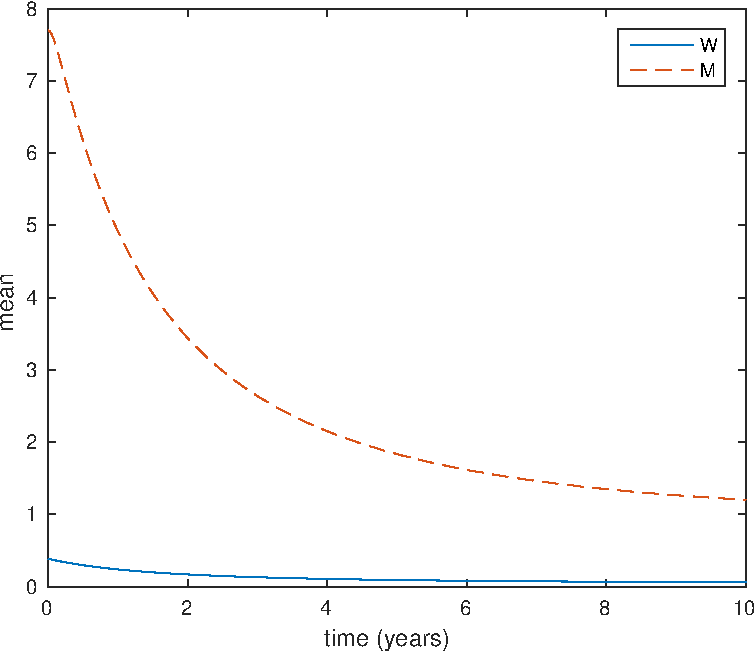
\includegraphics[height=5cm]{WM_1950s_omega=40per.pdf}\\
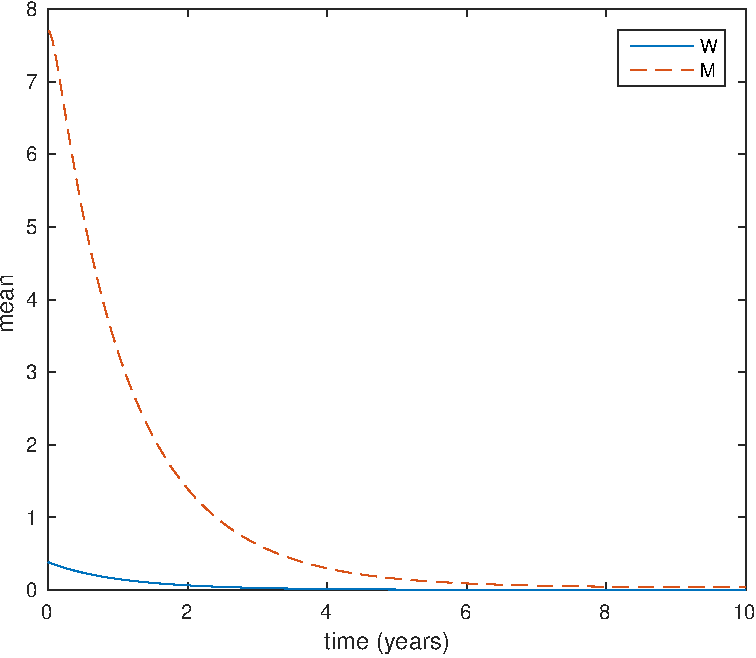
\includegraphics[height=5cm]{WM_1950s_omega=80per.pdf}
\end{array}$
\caption{The mean worm burden ($W$) and mf count per 20$\mu$l of blood ($M$) over time after an introduction of bednets at 40\% coverage to a population with equilibrium prevalence of $50\%$. Top: $\omega=0.4$. Bottom: $\omega=0.8$.}
\label{fig:WMs}
\end{center}
\end{figure} 
\begin{figure}[h]
\begin{center}
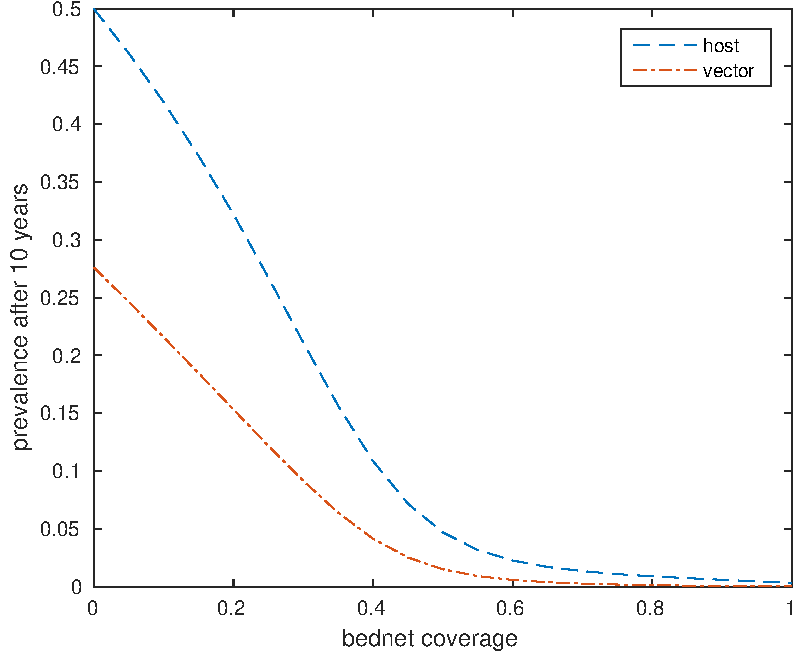
\includegraphics[height=5cm]{10yearprev_1950s_bednets.pdf}
\caption{The estimated host prevalence (from mf count $M$) after 10 years of fixed bednet coverage, with the proportion of bednet usage ranging between $0$ and $1$, for a population with an equilibrium prevalence of $50\%$.}
\label{fig:10year}
\end{center}
\end{figure} is $50\%$, reflecting the conditions in The Gambia in the 1950s \cite{rebollo2015}, which translates as a mean mf count per 20$\mu$l of blood of $7.70$. The model predicts that introducing bednets at $40\%$ coverage to this setting could decrease the mf count, $M$, to under $20\%$ of it's original level within 10 years (Fig. \ref{fig:WMs}); a coverage of $80\%$ could bring it down even further to near $0$. These results are following just a scale up of bednet usage, with no consideration for MDA, but represent large decreases in mean worm burden and mf count. The average lifespan of an adult worm used in the model is approximately 8 years, so considering a 10 year period allows demonstration of the full affect of the bednets. 

Although mean worm burden, $W$, and mf count, $M$, are descriptive measures of helminth infection levels in a host population, much epidemiological discussion is focused around the prevalence. This is because the number of infected individuals is informative when planning treatment and morbidity management programs, as well as for setting and communicating public health goals.

Fig. \ref{fig:10year} shows the effect differences in bednet coverage could have on host and vector prevalence after 10 years, assuming no loss of efficacy of the bednets over time due to loss of insecticide potency or degradation of the net material. High levels of coverage (50\% or higher) could result in a host prevalence of less than 5\%. Host prevalence is higher than the vector prevalence because of the long lifespan of human hosts, particularly due to the very slow recovery rate in the absence of treatment caused by adult worms living more than 8 years on average. The introduction of bednets subdues infection by reducing transmission in both directions, causing increased vector death and lowering the infectious bite rate.

\subsection{Transmission in other settings}

A prevalence of 50\% is representative of a high transmission setting, so it would follow that any kind of intervention is likely to make a substantial impact, although elimination would be more difficult. It is informative to consider how usage of bednets could influence prevalence in areas of lower transmission. Comparing ten year program outcome predictions for different combinations of bednet coverage and \begin{figure}[h]
\begin{center}
\includegraphics[height=5cm]{heatmap_prev.pdf}
\caption{Prevalence after 10 years for combinations of bednet coverage and equilibrium host prevalence in the absence of vector control according to bednet parameters given in Table \ref{table:param}.}
\label{fig:heat_prev}
\end{center}
\end{figure}
\begin{figure}[h]
\begin{center}
\includegraphics[height=5.5cm]{interrupttrans.pdf}
\caption{Categorisation of whether the WHO threshold for interrupted transmission (prevalence of less than 1\%) has been met after 10 years of bednet coverage ranging between 0 and 1 and equilibrium host prevalences between 0.05 and 0.6.}
\label{fig:interrupt}
\end{center}
\end{figure} baseline host prevalence (Fig. \ref{fig:heat_prev}) shows that bednets can make a difference even in areas with much lower transmission.

For bednet coverage of 60\% or higher it is possible to bring prevalence below 5\% over a ten year period, irrespective of initial prevalence. For equilibrium conditions of less than 25\% host prevalence, the same result can be achieved with only 30\% of people sleeping under bednets. In low transmission settings high bednet coverage isn't required; a coverage of 15 or 20\% could still result in large relative reductions of prevalence.

WHO Guidelines for LF elimination define a threshold prevalence of 1\% for ceasing MDA programs and moving into the monitoring phase \cite{GPELF}. Transmission assessment surveys (TAS), which look at LF antibody levels, are then carried out to verify interrupted transmission. If a setting already has prevalence below 1\% then only the monitoring phase is required. Fig. \ref{fig:interrupt} shows that the model predicts this would in fact be possible for all realistic transmission levels, with the required bednet coverage depending on baseline host prevalence. In low endemicity settings a bednet coverage of between 40 and 60\% could be sufficient.
\begin{figure}[h]
\begin{center}
\includegraphics[height=5cm]{heatmap_prev_pess.pdf}
\caption{Prevalence after 10 years for combinations of bednet coverage and equilibrium host prevalence in the absence of vector control according to the most pessimistic estimations for bednet influence: probability of bednet-induced death, $\nu=0.05$, and probability of successful feeding in the presence of bednet, $\sigma=0.6$.}
\label{fig:inter_pess}
\end{center}
\end{figure}
\begin{figure}[h]
\begin{center}
\includegraphics[height=5.5cm]{paramsensitivity2.pdf}
\caption{Vector prevalence and population size for different combinations of success ($\sigma$) and death ($\nu$) probabilities. Height of surface represents population size and colour represents equilibrium vector prevalence. Probability of vector infection given one successful bite is $p=0.185$. Bednet coverage: $\omega=0.4$.}
\label{fig:params}
\end{center}
\end{figure}

\subsection{Bednet efficacy}

Reductions in prevalence are governed by the parameters describing the efficacy of bednets as a tool for preventing transmission, specifically the probabilities of death ($\nu$) or success ($\sigma$) given an attempt to feed in the presence of a bednet. The chosen values for the model are the same as those used in Le Menach et al (2007) \cite{le2007}, but these represent the more positive end of the estimated regions given: $\nu=0.3$ and $\sigma=0.1$. Taking the worst case, $\nu=0.05$ and $\sigma=0.6$, results in much a lower predicted effect (Fig. \ref{fig:inter_pess}). With these pessimistic parameters no amount of bednet coverage can bring the prevalence down to under $1\%$, but it is probable that the true values will begin close to the optimistic values for new bednets and then will worsen over time as bednet efficacy decreases with use.

Using the distribution model it's possible evaluate the impact of a variety of combinations of $\nu$ and $\sigma$ on vector prevalence and population size (see Fig. \ref{fig:params}). Decreasing $\sigma$ makes it less likely that a vector will feed on any given attempt, meaning death has a higher chance of occurring before feeding, but this effect is relatively small due to fast feeding rates. In contrast, increasing efficacy of the bednet insecticide results in larger relative decreases in vector prevalence and population size; variations in the probability of a vector dying upon contact with a bednet, $\nu$, have the larger effect.

\section{Discussion}

\subsection{Model evaluation}

By explicitly considering the influence of bednets on mosquito feeding we have developed a novel model for lymphatic filariasis transmission in the presence of LLINs. We combined concepts from previous LF transmission models, such as the EPIFIL model \cite{norman2000}, and malaria-specific models concerning vector control \cite{le2007,killeen2016} to build a more complete picture of the potential use of bednets in the drive for LF elimination. In particular, modelling the gonotrophic cycle of adult female mosquitoes allows tracking of vector infection and bednet interaction, giving insights into how both increased vector death rates and delays in feeding due to bednets affect prevalence.

When model predictions are compared to a scenario in The Gambia, where halted LF transmission in the absence of MDA is attributed to bednets distributed by malaria control programs \cite{rebollo2015}, we see that just 10 years of medium-level bednet coverage can lead to significant decreases in the baseline 50\% prevalence. It is apparent that the model is able to qualitatively reproduce real-world situations, although more detailed data on bednet coverage and prevalence in The Gambia over time would be needed to verify the quantitative predictive power. 

As previously discussed when examining the sensitivity of results to bednet parameters, the model does not consider the waning efficacy of bednets. The insecticide potency is likely to decrease over time, resulting in a lower effective death rate of vectors, and the structure of the net itself can lose integrity due to general wear and tear. The parameters used in the model reflect the expected efficacy of a new bednet and, as such, the results may be unduly optimistic; waning insecticide efficacy is likely to have the largest impact on predictions.

Further extensions to the model could incorporate the negative binomial force of infection to avoid losing information or accuracy during conversion of the mf count to host prevalence, as discussed in Equation \ref{eqn:negbin}; this would require data on the one-hit probability of a vector becoming infected following ingestion of a single microfilaria. Indoor residual spraying (IRS) is a type of vector control that has not been examined here but it could easily be included in the model through an additional death rate in the Fed class. After feeding mosquitoes will find somewhere nearby, usually indoors, to sit and digest; if IRS has been carried out inside the house in which a mosquito feeds then it can result in death at this stage, increasing the death rate.

\subsection{Impact}

The qualitative results of the model show that vector control, specifically use of bednets, could present a feasible strategy for a number of settings in the journey towards LF elimination. Concerns about the effective timescale of such measures should be partly alleviated by the marked decrease in microfilariae count mostly occurring in the first four years following application of bednets, shown for coverages of 40\% and 80\% in Fig. \ref{fig:WMs}; the remaining positive effects are translated into further reductions by the end of ten years. Although vector control is still slower to take effect than MDA programs, this model gives a more positive outlook on the progress that can be made in a relatively short period of time than recent studies \cite{norman2000}. Repeated MDA is expensive and usually run for at least 5 years before cessation of treatment, often followed by a small uptake of disease. Usage and efficacy of bednets are likely to wane over time without redistribution \cite{kweka2011}, but gradually and unlike the definitive cut off at the end of an MDA program. Despite the long lifespan of adult worms, often up to eight years, distribution and use of bednets could have a rapid effect on the levels of disease, with significant gains in the first year. 

It has been demonstrated that bednet coverage alone could feasibly be sufficient for reaching thresholds set by the WHO that define interrupted transmission. The ten year time frame is too long for the 2020 elimination targets, although there is the potential that some countries that have yet to begin MDA may find that existing bednet usage has already begun the elimination process. More data would be needed to verify such a model before rigorous conclusions could be made on the expected outcome of bednet-only elimination programs, but the prospect could be more plausible that previously expected. Bednet-driven programs would save money in comparison to MDA, with cross-disease effects benefiting the control and elimination of malaria in settings where both diseases are endemic.

%\begin{thebibliography}{1}
%\bibitem{WHO2016} Kermack W O, McKendrick A G, A contribution %to the mathematical theory of epidemics. Proc. R. Soc. A %1927;115:700?721. 
%\end{thebibliography}

%\bibliography{report}
\appendix
\section{Approximating $C$}    % Capa Apandice debe tener un tatulo corto.
The current form of $C$ doesn't give any intuitive understanding of the system, but it may be possible to derive some using approximations. To begin with, since slow relative death rates give $\delta<<\pi_k$ for all $k=1,\dots,4$ then we get that
\begin{equation}
\frac{\pi_k}{\pi_k+d} \approx 1 - \frac{\delta}{\pi_k}
\end{equation}
and hence, neglecting higher order terms in $\delta$,
\begin{eqnarray}
C &=& \frac{\pi_1\pi_2\pi_3\pi_4p_1}{(\pi_2(p_1+p_2)+\delta)(\pi_3+\delta)(\pi_4+\delta)(\pi_1+\delta)} \\
&\approx& \frac{\pi_2p_1}{\pi_2(p_1+p_2)+\delta}\Big(1-\frac{\delta}{\pi_1}-\frac{\delta}{\pi_3}-\frac{\delta}{\pi_4}\Big)\\
&\approx& \frac{p_1}{p_1+p_2} \Big(1-\frac{\delta}{\pi_2(p_1+p_2)}\Big)\\&& \mbox{ }\times \Big(1-\frac{\delta}{\pi_1}-\frac{\delta}{\pi_3}-\frac{\delta}{\pi_4}\Big)
\end{eqnarray}
Now, we have that if $\pi_2>>\pi_k$ for all $k\neq 2$ then
\begin{eqnarray}
C \approx \frac{p_1}{p_1+p_2}\Big(1-\delta\Big(\frac{1}{\pi_1} + \frac{1}{\pi_2} +\frac{1}{\pi_3} + \frac{1}{\pi_4}\Big)\Big)\,,
\end{eqnarray}
which is the product of the probability of feeding rather than dying upon contact with a bednet and the probability of surviving a full generation given the natural death rate.

With chosen values $\pi_2 = 5$ and $\pi_k=5/3$ for $k\neq 2$ and a bednet coverage of $\omega=0.4$ we get that $C=0.53300$ and the approximation, $\tilde{C}=0.53312$, giving only a 2.29\% error (to 3.s.f). One generational cycle is taken to be 2 days in length.

\section{Vector prevalence estimation figures}

\begin{figure}[h]
\begin{center}$
\begin{array}{c}
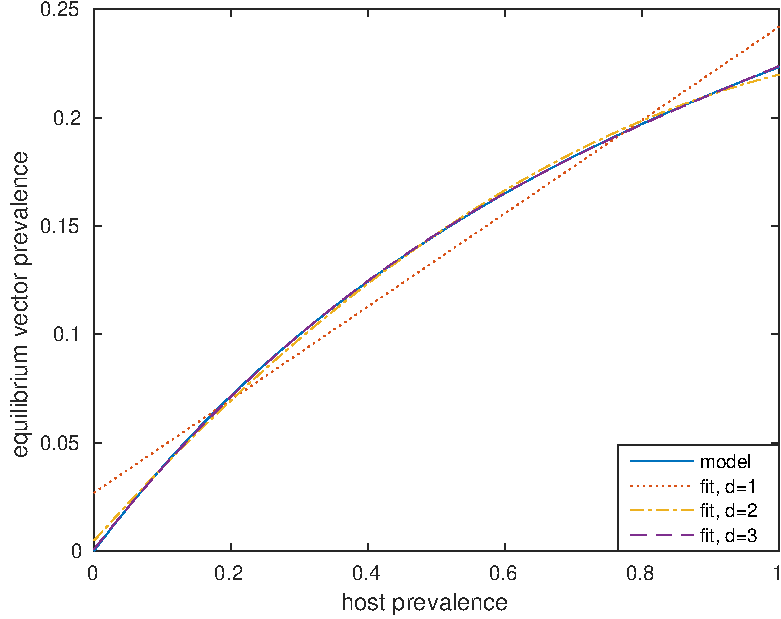
\includegraphics[height=5cm]{polyfit_prev_prev.pdf}\\
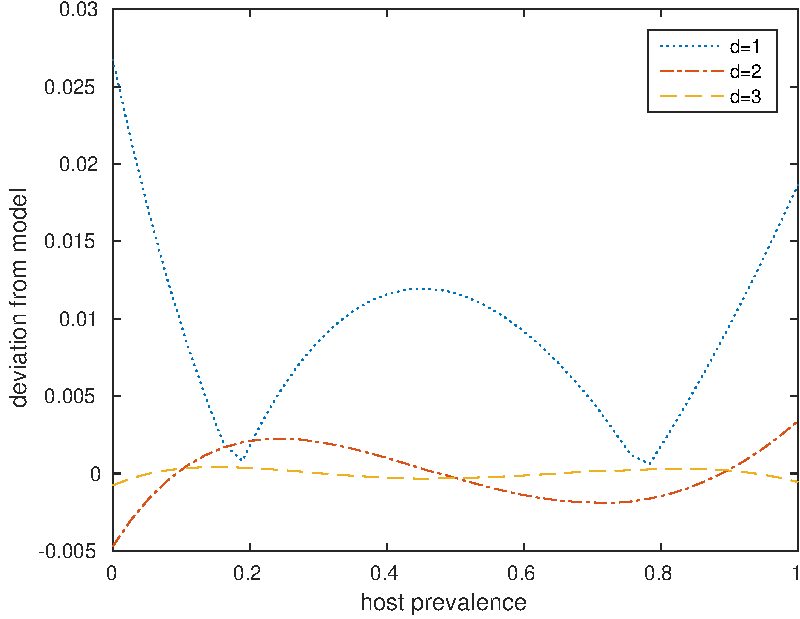
\includegraphics[height=5cm]{polyfit_prev_prev_deviation.pdf}
\end{array}$
\caption{Polynomial fits to the equilibrium vector prevalence as a function of host prevalence, for degree $d=1,2,3$, $\omega=0.4$. Top: The fitted curves compared to the model curve. Bottom: The deviation of each fit from the model.}
\label{fig:polyfit}
\end{center}
\end{figure}

%\bibliographystyle{elsarticle-harv}
\bibliographystyle{unsrt}
\bibliography{report}

\end{document}

%%
%% End of file `ejemplo latex RIAI.tex'.